\chapter{結果と考察}
本章では,シミュレーション,評価実験,アンケートの結果とその考察について述べる.

\section{シミュレーション結果と考察}
シミュレーションの結果,Pillowでは一定時間経過後のリマインダーが24回,ソースコード変更量の検知が32回呼び出され,Pipenvでは一定時間経過後のリマインダーが24回,ソースコード変更量の検知が451回呼び出されることがわかった.
Pipenvのシミュレーション結果を図\ref{sim1},Pillowのシミュレーション結果を図\ref{sim2}に示す.
水色の折れ線がドキュメントのコミット数,オレンジ色の折れ線がソースコードのコミット数,紫色の点がC2の呼び出し,緑色の点がC4の呼び出しを表す.
C3については呼び出しがなかった.
また,シミュレーション結果を図に表す時,各機能の呼び出しを日単位でまとめているため,実際の呼び出し回数より少なく表示されている.

\begin{figure}[H]
    \centering
    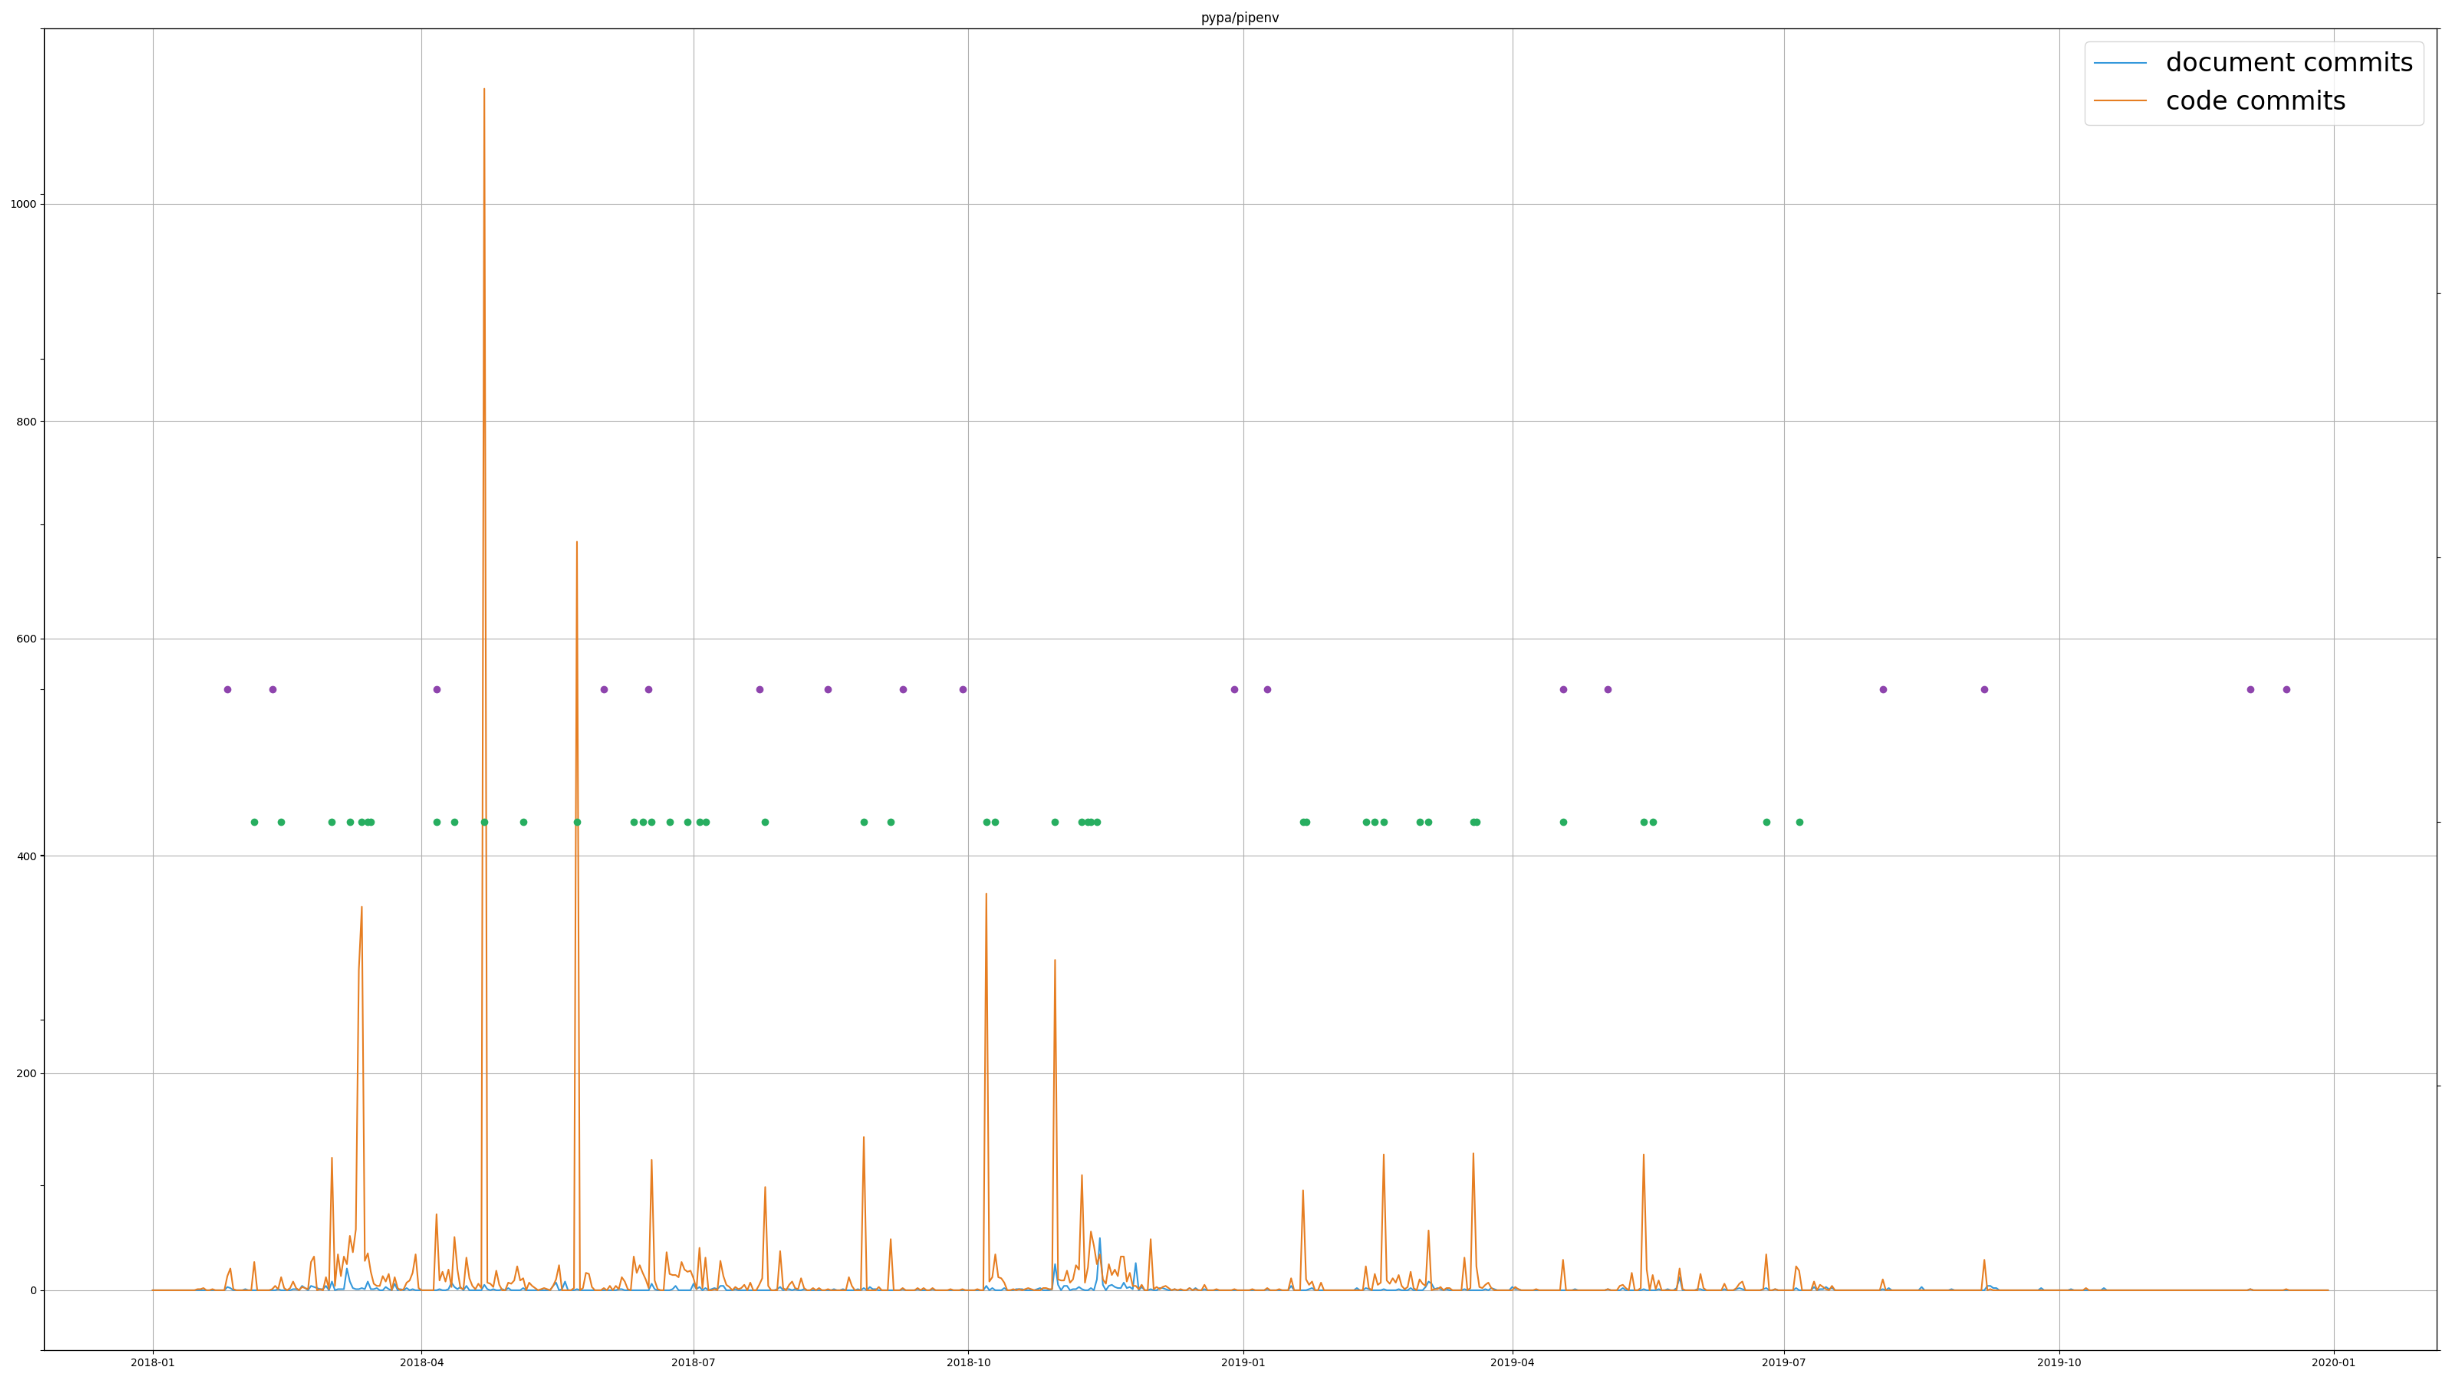
\includegraphics[width=14cm]{images/sim1.png}
    \caption{Pipenvのシミュレーション結果}
    \label{sim1}
\end{figure}

\begin{figure}[H]
    \centering
    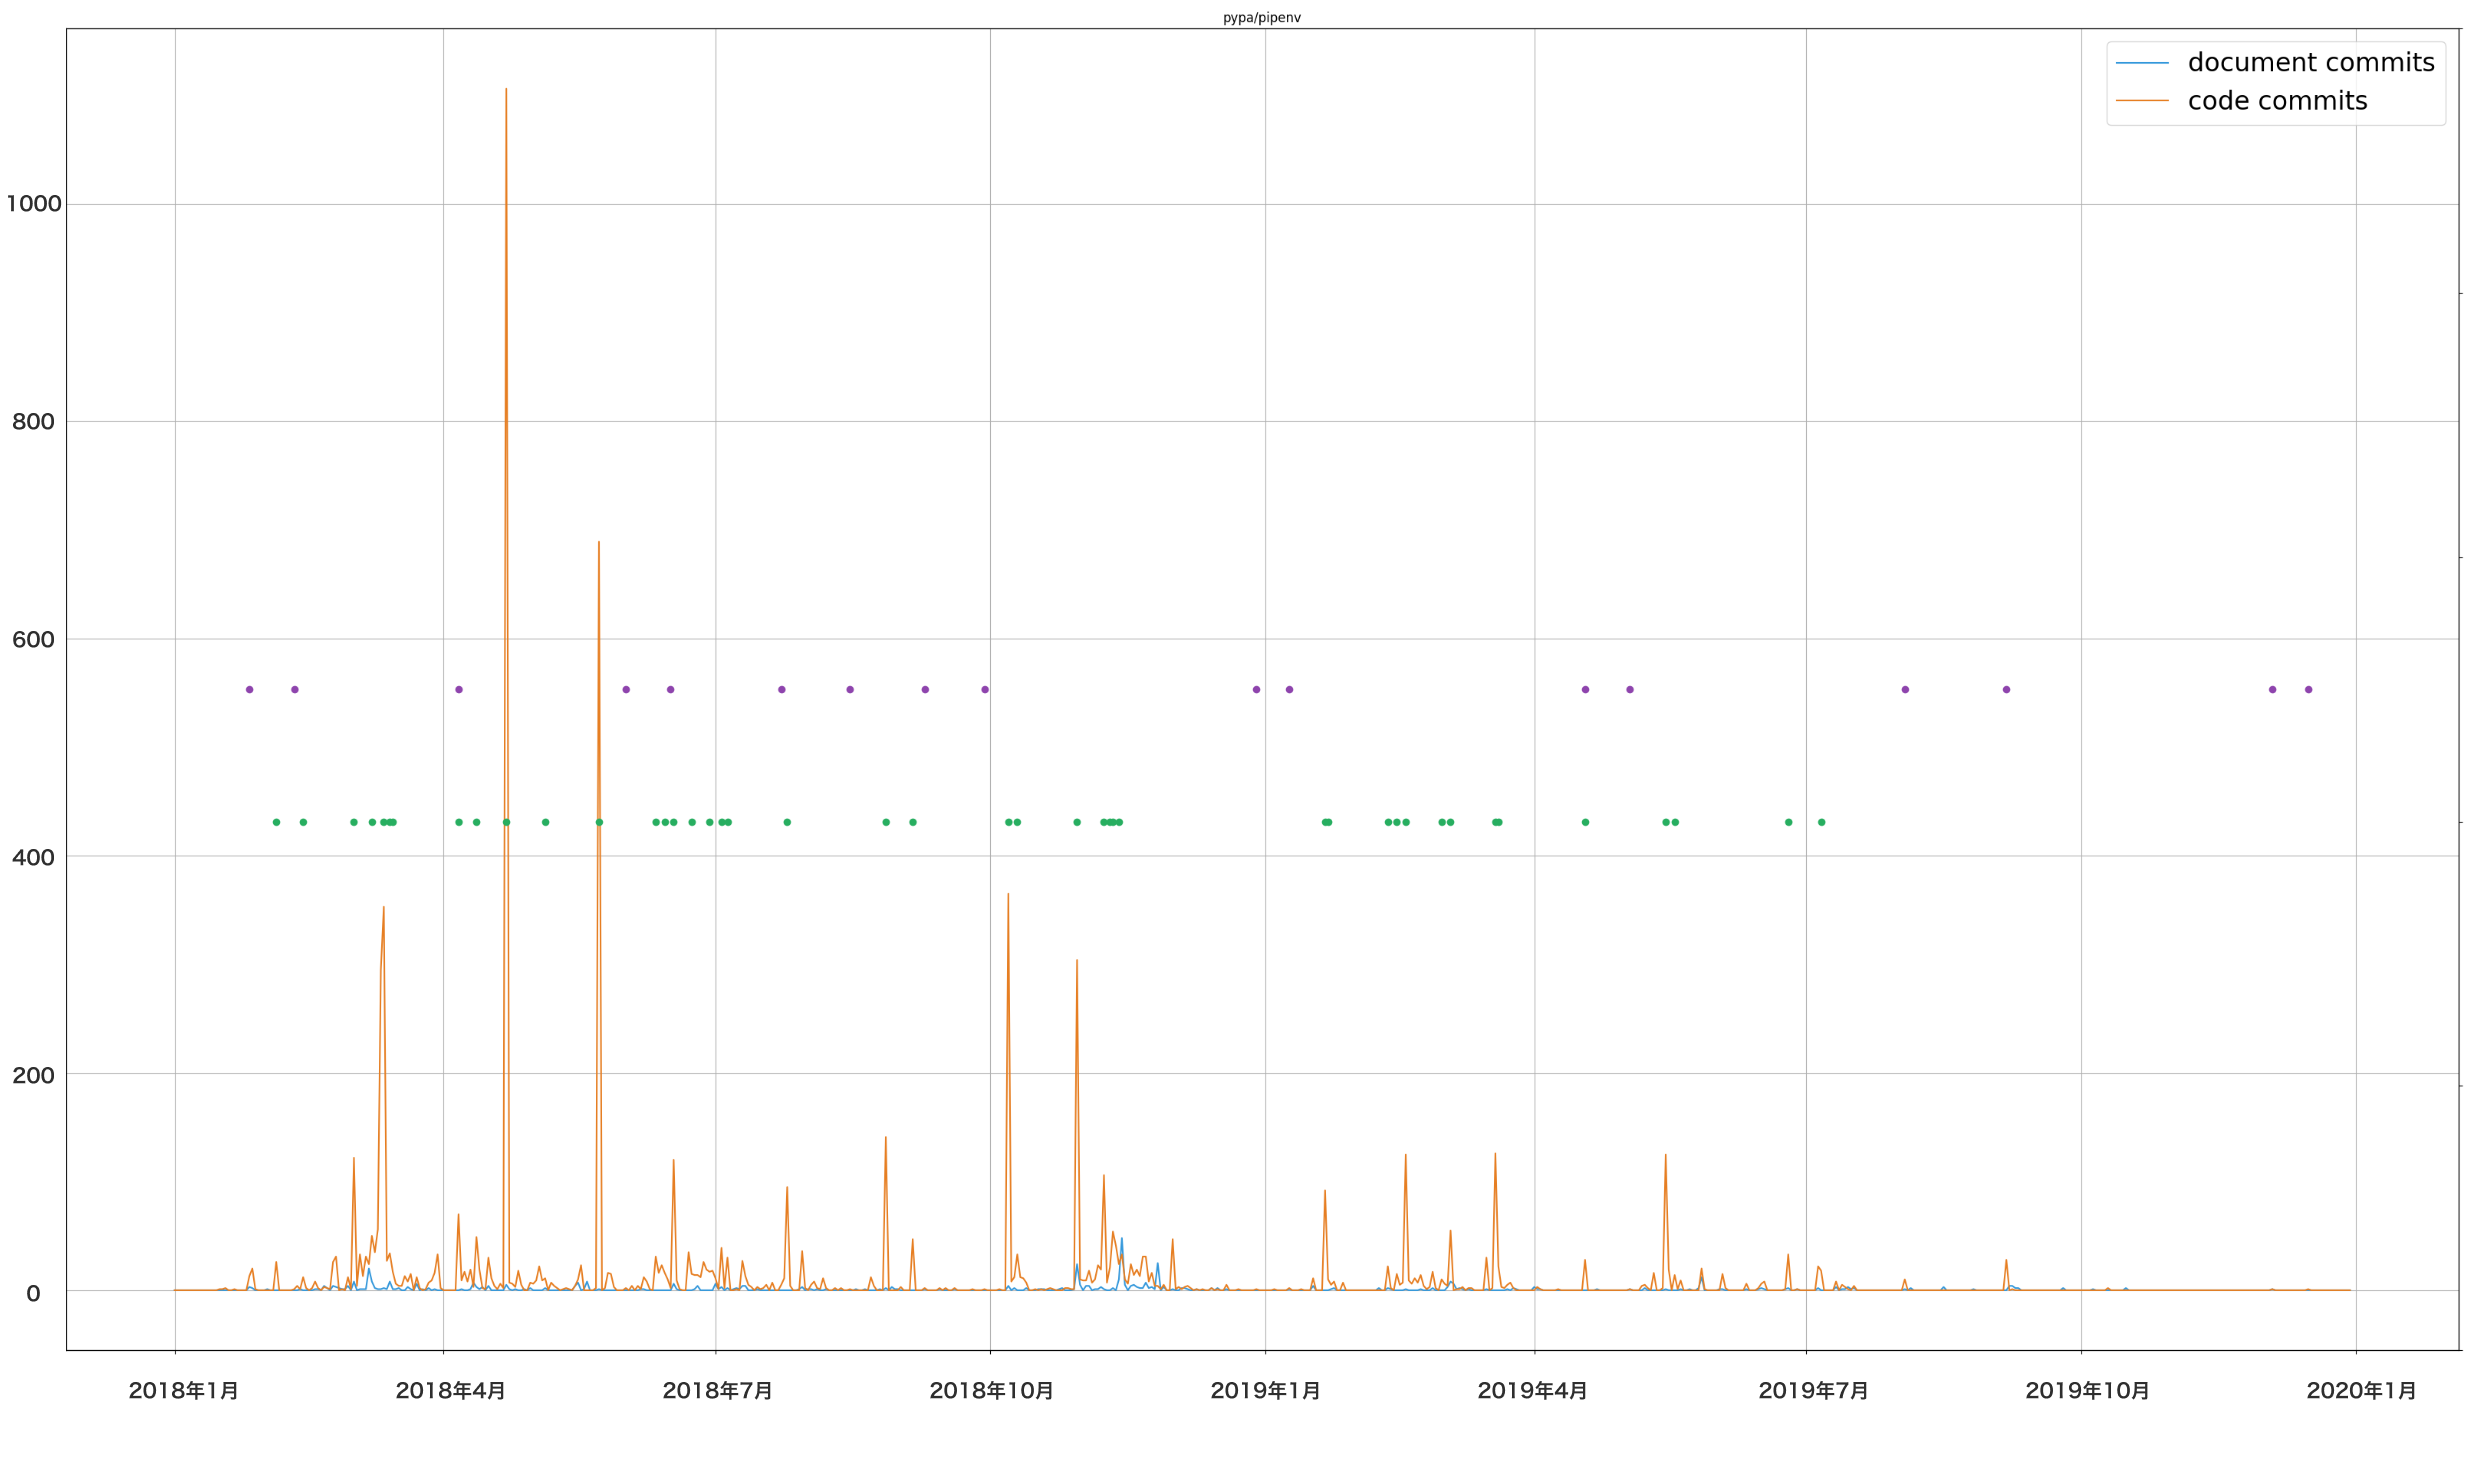
\includegraphics[width=14cm]{images/sim2.png}
    \caption{Pillowのシミュレーション結果}
    \label{sim2}
\end{figure}

図\ref{sim1}より,Pipenvでは2019年以降に積極的な開発が行われていないため,ドキュメントとソースコードのコミット数が減少傾向にあることがわかる.
そのため,ドキュメントとソースコードの乖離が起こることは少ないが,それでも通知を出してしまっている結果となっているため,
ドキュメントやソースコードで機能の追加や修正に全く関係のないコミットが通知を出さないように改良する必要があることが判明した.

以上のシミュレーション結果より,ドキュメントとソースコードの乖離リスクが検知されたときに通知を出すことで,乖離の抑制に役立つ可能性があることが判明した.
一方で,精度の高い検知を行うためには,さらなる改善を加えないといけないことがわかった.
また,様々なプロジェクトでシミュレーションを行うことのできるシミュレータの改善や,プロジェクト規模に合わせた各種パラメータの自動調整などをする必要があると考える.


\section{実験結果と考察}
\ref{plan}節で示した実験計画に従って評価実験を行った.
以下では,実験協力者2名について,それぞれのタスクの取り組みや,ドキュメントとソースコードの乖離検知をしたときの行動を詳細にまとめる.

\subsection{前半に提案ツールを使用した実験協力者}
前半に提案ツールを使用した実験協力者(以下,実験協力者Aと呼ぶ)の行動と乖離検知の流れを図\ref{usera}に示す.
\begin{figure}[H]
    \centering
    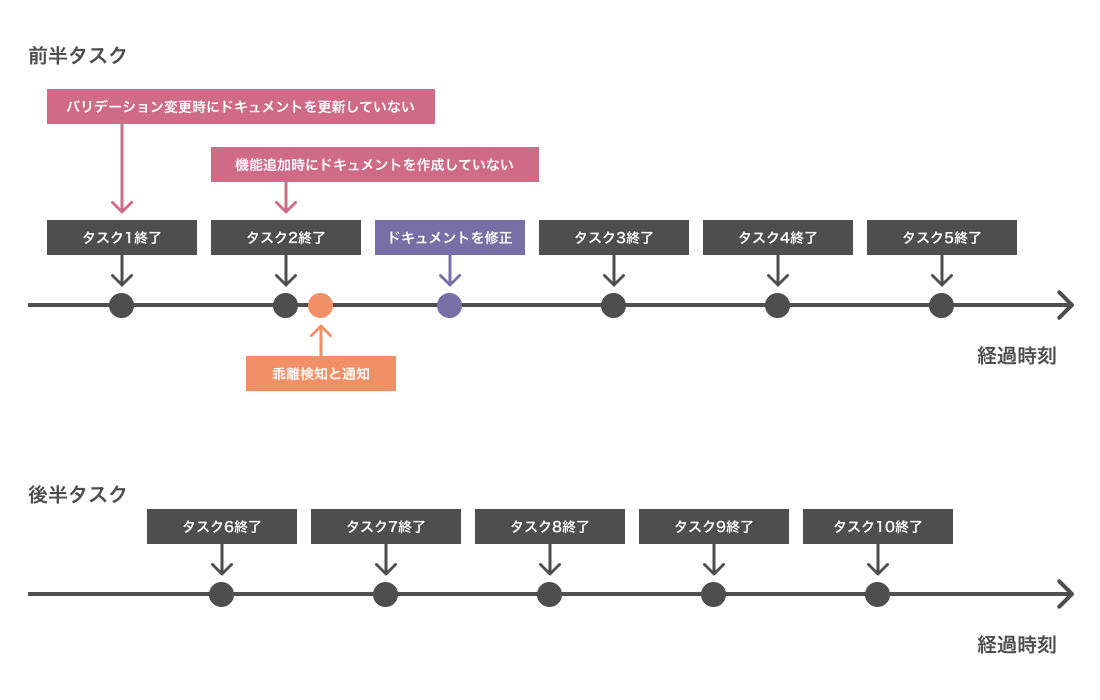
\includegraphics[width=8cm]{images/UserA.png}
    \caption{前半に提案ツールを使用した実験協力者の行動と乖離検知の流れ}
    \label{usera}
\end{figure}

実験協力者Aは,タスク1ではドキュメントを更新せずにソースコードの追加のみを行っていた.
このとき,提案ツールではバリデーションの変更からSwagger形式のドキュメントとソースコードの乖離を検知することができないため,
乖離検知を行わず,通知を送ることはなかった.
次に,新たな機能を作成するタスク2を終えたときに,提案ツールが乖離検知を行ったため,実験協力者Aに「[C1]: ドキュメントに無い機能であるget\_users を作成しています」と通知を送った.
図\ref{notification1}は,実際に実験協力者Aに通知を行った時のメッセージである.

\begin{figure}[H]
    \centering
    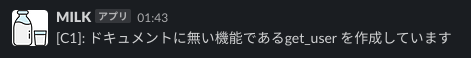
\includegraphics[width=10cm]{images/notification1.png}
    \caption{乖離検知をしたときに実験協力者Aに通知を送ったときのメッセージ}
    \label{notification1}
\end{figure}

その後の後半タスクでは,前半に乖離検知の通知を受け取ったことを受けて,タスクに取り組むときは,ドキュメントとソースコードの両方を追加・修正しており,
ドキュメントとソースコードが乖離することはなかった.

\subsection{後半に提案ツールを使用した実験協力者}
後半に提案ツールを使用した実験協力者(以下,実験協力者Bと呼ぶ)の行動と乖離検知の流れを図\ref{userb}に示す.
\begin{figure}[H]
    \centering
    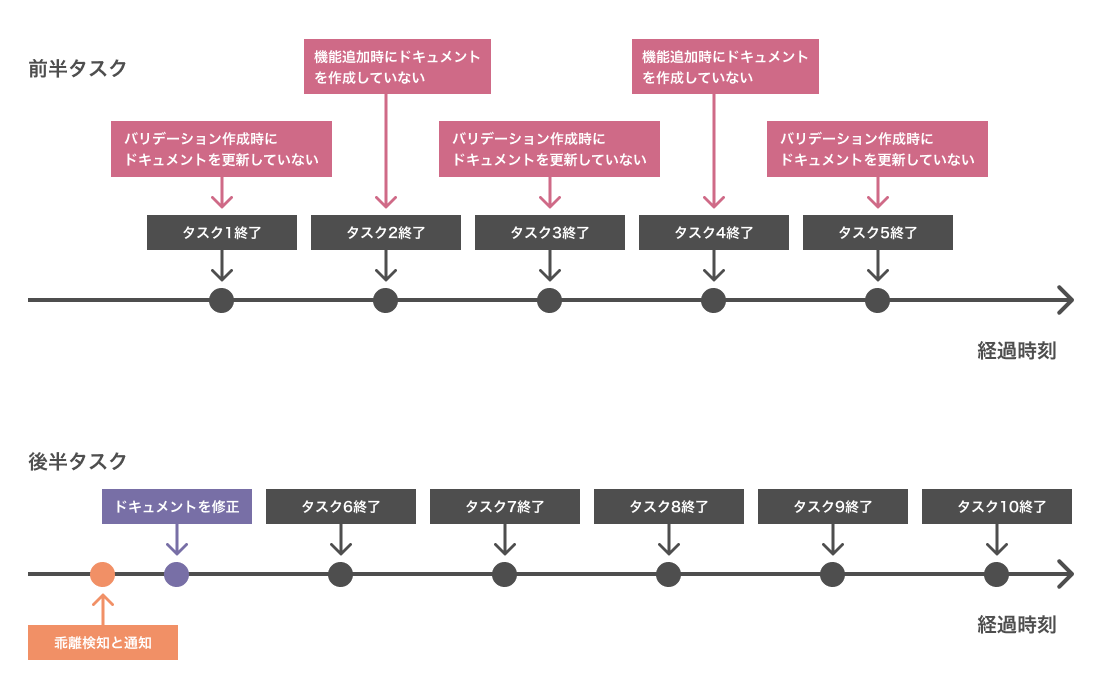
\includegraphics[width=8cm]{images/UserB.png}
    \caption{後半に提案ツールを使用した実験協力者の行動と乖離検知の流れ}
    \label{userb}
\end{figure}

実験協力者Bは,前半タスクをこなす間,一度もドキュメントに触れることなくソースコードの追加を行っていた.
後半タスク開始時に,ドキュメントとソースコードの乖離検知が行われたため,実験協力者Bに「[C1]: ドキュメントに無い機能であるget\_user get\_users\_child を作成しています」と通知を送った.
図は\ref{notification2},実際に実験協力者Bに通知を行った時のメッセージである.

\begin{figure}[H]
    \centering
    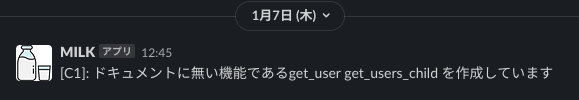
\includegraphics[width=10cm]{images/notification2.png}
    \caption{乖離検知をしたときに実験協力者Aに通知を送ったときのメッセージ}
    \label{notification2}
\end{figure}

ここで,タスク6を開始する前に,実験協力者Bはドキュメントの更新を行ったため,ドキュメントとソースコードの乖離が抑制された.
その後,後半タスクが終了するまでドキュメントとソースコードが乖離することはなかった.

\subsection{実験結果の考察}
上記では実験協力者2名について,それぞれのタスクの取り組みや,ドキュメントとソースコードの乖離検知をしたときの行動を詳細にまとめた.
2名とも,乖離検知の通知を受け取った直後に,ドキュメントの修正を行っており,全タスク終了時にはドキュメントとソースコードが乖離することはなかった.
このことから,RESTful APIの開発において,提案ツールはドキュメントとソースコードの乖離抑制に一定の効果が見込めることが判明した.
一方で,実験協力者Aのタスク1において,バリデーションを修正したがドキュメントを更新しなかったことについて,
乖離を検知できなかったため,提案ツールの性能を向上させる必要があると考えられる.

\section{アンケート結果と考察}
実施したアンケートを付録\ref{survey}に示す.
実験協力者2名に対し,Slackからの通知を受け取ったことで,ドキュメントを更新しないといけないと感じたかという質問に対し,1名が「とても思った」,1名が「やや思った」と回答した.
回答結果を図\ref{q1}に示す.
\begin{figure}[H]
    \centering
    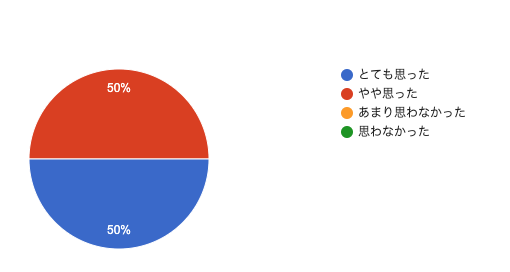
\includegraphics[width=10cm]{images/q1.png}
    \caption{アンケート結果: Slackからの通知を受け取ったことで,ドキュメントを更新しないといけないと感じたか}
    \label{q1}
\end{figure}

また,ドキュメントの更新を忘れてしまったとき,通知は必要だと感じるかという質問に対し,2名が必要であると回答した.
回答結果を図\ref{q2}に示す.
\begin{figure}[H]
    \centering
    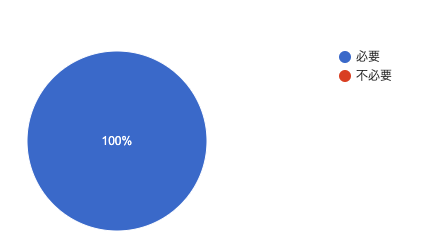
\includegraphics[width=10cm]{images/q2.png}
    \caption{アンケート結果: ドキュメントの更新を忘れてしまったとき,通知は必要だと感じるか}
    \label{q2}
\end{figure}

Slackから受け取った通知内容で改善して欲しいところはあるかという質問に対して,以下のような回答を得た.
\begin{itemize}
    \item 通知内容が簡素に感じた
    \item もっと詳細を教えて欲しい
\end{itemize}

以上のアンケート結果より,提案ツールはドキュメントとソースコードの乖離の抑制に効果を感じていることがわかった.
一方で,通知内容を改善し,開発者に親しみやすいように改良を加えることで,より使いやすいツールになることが判明した.